\documentclass[UTF8,a4paper,11pt]{ctexart}
\usepackage[a4paper,margin=2.2cm]{geometry}
\usepackage{amsmath,amssymb,booktabs,graphicx,float,caption,hyperref,xcolor}
\usepackage{array,tabularx,longtable}
\hypersetup{colorlinks=true,linkcolor=blue,urlcolor=blue,citecolor=blue}
\graphicspath{{../figures/generated/}}
\setlength{\parindent}{2em}
\setlength{\parskip}{0.25em}
\captionsetup{font=small,labelfont=bf}
\newcommand{\keywords}[1]{\par\noindent\textbf{Keywords: }#1}
\title{基于图神经网络的多机器人协同路径规划与避碰方法研究}
\author{研究论文初稿}
\date{\today}

\begin{document}
\maketitle

\begin{abstract}
Background: Multi-robot navigation requires goal reaching, coordination, and collision avoidance under changing interaction topology. Methods: We formulate robots as nodes in a dynamic communication graph and learn shared local velocity policies using message passing, five-dimensional relative-motion edge features, a joint imitation-and-safety objective, and an external safety filter. The policies are compared with A*, ORCA-style, RVO-style, and independent MLP baselines on four map families, 5--40 robots, and 30 unseen seeds per configuration; ROS 2, Gazebo, and RViz2 integration is also tested. Results: With safety filtering, Graph Transformer obtains a strict no-physical-collision success rate of 1.000 at 10 robots, while GNN obtains 0.967, 0.958, and 0.708 at 5, 10, and 20 robots, respectively. At 40 robots, strict success decreases to 0 for GNN and 0.017 for Graph Transformer, and control time increases with population size. Conclusions: Dynamic graph policies provide an effective and computationally practical solution in low-to-medium density settings, but the observed high-density degradation shows that stronger safety-constrained training and additional real-robot validation are still required.
\end{abstract}

\noindent\textbf{关键词：}多机器人；图神经网络；协同路径规划；碰撞避免；动态通信图；ROS 2
\keywords{multi-robot systems; graph neural networks; cooperative path planning; collision avoidance; dynamic interaction graphs; ROS 2}

\noindent\textbf{中文摘要：}本文研究动态通信图下的多机器人协同路径规划与避碰问题，提出带有相对运动边特征、联合训练目标和安全过滤器的共享局部策略，并对 GNN、Attention-GNN 和 Graph Transformer 进行多规模测试。实验覆盖四类地图和 5--40 个机器人。结果表明，Graph Transformer 在 10 个机器人时严格无碰撞成功率达到 1.000，GNN 在 5--20 个机器人范围内兼顾较好的成功率和控制时间；当规模达到 30--40 个机器人时，安全性明显下降。本文同时完成 ROS 2、Gazebo 和 RViz2 的接口与可视化验证。

\section{引言}
多机器人协同路径规划的目标是在共享环境中为多个机器人生成满足目标到达、运动约束和安全间距要求的运动策略。与单机器人规划相比，多机器人系统的状态维度随机器人数量增加，机器人之间的相互影响也随时间变化。集中式搜索容易受到组合状态空间的影响，完全独立的局部策略又难以利用邻居信息。

图神经网络（Graph Neural Network, GNN）能够通过节点和边表示实体及其关系，并利用消息传递聚合邻居信息。因此，将机器人群体建模为动态图，可以在保持参数共享的同时表达局部交互关系。本文研究以下问题：在相同观测、动作限制和终止条件下，局部通信图是否能够帮助学习策略获得更好的多机器人协同行为？通信范围和安全过滤如何影响成功率、碰撞事件和计算开销？

本文的主要贡献包括：
\begin{enumerate}
  \item 设计相对运动感知的动态图策略，将归一化相对位置、相对速度与接近速度组成五维边特征，通过共享消息传递建模机器人交互，支持可变规模的机器人团队；
  \item 设计兼顾安全的学习与执行机制，联合动作模仿、一步间距、目标进度与平滑损失，并在执行阶段引入可选的外部两两安全过滤器，独立评估其作用与神经策略本身的效果；
  \item 在四类地图、5--40 个机器人与 30 个未见种子上开展可复现验证，通过经典与神经基线对比及图结构、通信半径和安全层消融识别密度边界，并以统一实验框架和 ROS~2/Gazebo/RViz2 集成支撑验证。
\end{enumerate}

\section{相关工作}
\subsection{传统路径规划}
A* 由 Hart 等提出，通过启发式函数在离散网格上搜索低代价路径，优点是静态地图上的完备性和可解释性，缺点是多机器人联合搜索的组合复杂度高，且单机器人路径需要额外协调\cite{hart1968}。Fiorini 和 Shiller 提出速度障碍思想，通过预测相对运动判断候选速度是否会导致碰撞；其优点是几何意义清晰，缺点是对局部观测、时间窗和参数较敏感\cite{fiorini1998}。Long 等将深度强化学习用于去中心化多机器人避碰，使每个机器人依据局部观测独立决策，优点是推理阶段无需集中式联合搜索，缺点是训练分布外的密集交互容易产生碰撞\cite{long2018orcamarl}。Thumiger 和 Deghat 面向 UAV 提出多智能体深度强化学习避碰方法，改善了实际飞行约束下的分散决策，但其场景和动力学假设不直接覆盖地面机器人\cite{thumiger2022uav}。

\subsection{学习型多机器人规划}
Diao 等提出基于图神经网络的机器人路径规划方法，用图结构编码空间关系，优点是能显式利用邻居信息，缺点是论文场景规模和跨地图泛化仍有限\cite{diao2024gnn}。He 等提出图注意力网络与分层运动规划相结合的多机器人导航方法，通过注意力选择重要邻居，优点是可抑制无关交互，缺点是注意力训练稳定性和计算开销需要权衡\cite{he2023ganav}。Goarin 和 Loianno 将 GNN 用于去中心化目标分配，使机器人共享结构化表示完成任务匹配，优点是适合可变规模群体，缺点是目标分配并不等价于连续避碰\cite{goarin2024assignment}。Yang 等将 GNN 与 PPO 结合用于多 UAV 协同路径规划，优点是能够利用长期回报优化协同策略，缺点是强化学习训练成本和仿真到现实迁移风险较高\cite{yang2025uav}。

Serra-Gómez 等学习可扩展的多机器人通信策略，在通信选择和避碰之间进行联合优化，优点是减少不必要通信，缺点是通信策略对训练分布和传感器假设敏感\cite{serragomez2023communication}。Komol 等在受限通道中使用课程强化学习逐步增加任务难度，优点是有助于学习狭窄通道行为，缺点是课程设计会影响复现性和泛化范围\cite{komol2025curriculum}。Feng 等引入物理先验强化学习约束多智能体避碰，优点是把动力学和安全知识纳入优化，缺点是物理先验设计和训练实现较复杂\cite{feng2024physics}。Dergachev 和 Yakovlev 使用模型预测路径积分进行去中心化避碰，优点是具有显式滚动优化能力，缺点是在线采样带来的计算时间随机器人数量增加\cite{dergachev2024mppi}。Parooei 等使用半监督深度强化学习处理复杂环境中的多智能体路径规划，优点是减少完全标注数据需求，缺点是伪标签质量会影响闭环性能\cite{parooei2023semisupervised}。

在应用型研究中，Niu 等将数据驱动多智能体强化学习用于多船避碰，展示了通信和协同决策的价值，但水面船舶动力学与本文二维地面机器人模型不同\cite{niu2023ship}。Xu 等研究多智能体编队和避碰，通过强化学习同时维持队形与安全间距，优点是任务目标更丰富，缺点是编队约束会限制自由路径规划\cite{xu2024formation}。Wang 等加入通信机制解决多船协同导航，优点是能表达意图交换，缺点是对通信可靠性要求较高\cite{wang2025ships}。Teng 等提出改进神经网络-DWA 的双层多机器人规划系统，优点是保留局部规划器的可解释性，缺点是网络与规则层之间的耦合参数较多\cite{teng2025dual}。Alwafi 等构建并评估多机器人路径规划图算法，优点是图结构便于表达任务关系，缺点是图搜索在高密度连续控制中仍可能产生较大开销\cite{alwafi2025graph}。Zhang 等将生物启发神经网络用于变电站巡检机器人动态规划，优点是面向具体巡检约束，缺点是应用场景专用性较强\cite{zhang2024glasius}。

从安全控制角度看，Abdulghafoor 和 Bakolas 研究带有碰撞保证的多智能体目标跟踪，优点是安全性质具有理论表述，缺点是目标跟踪假设与复杂障碍物导航不同\cite{abdulghafoor2023tracking}。Bechlioulis 等提出带自适应性能和避碰的分布式包围控制，优点是具有分布式控制稳定性分析，缺点是控制目标不是一般意义上的最短路径规划\cite{bechlioulis2024containment}。Yang 等的综述系统比较了多机器人碰撞规避协调方法，指出规则方法可解释但适应性有限，学习方法灵活但缺少安全保证\cite{yang2025survey}。本文因此采用“动态图学习策略加外部安全过滤”的折中结构：GNN 负责学习协同运动模式，过滤器负责处理近距离闭合风险，并用严格物理碰撞指标分别评价两者效果。该结构与现有研究的区别在于同时报告图结构、注意力模型、边特征、多规模压力测试和 ROS 2 实机接口链路，而不是只报告任务到达率。

\section{问题建模}
设机器人集合为 $\mathcal{V}=\{1,\ldots,N\}$，机器人 $i$ 的位置、速度和目标分别为 $p_i\in\mathbb{R}^2$、$v_i\in\mathbb{R}^2$ 和 $g_i\in\mathbb{R}^2$。根据通信半径 $R_c$ 建立动态图：
\begin{equation}
A_{ij}=\begin{cases}1,&i\ne j,\ \|p_i-p_j\|\le R_c,\\0,&\text{otherwise.}\end{cases}
\end{equation}
节点特征由目标相对位置、归一化速度、最近障碍物方向、最近障碍物距离和偏置项组成，维度为 8。策略输出二维局部速度 $u_i$，其模长限制为 $v_{max}=1.4$ m/s，位置更新为 $p_i^{t+1}=p_i^t+\Delta t u_i^t$，其中 $\Delta t=0.08$ s。当任意机器人对的距离小于 $d_s=0.72$ m 时，记为一次碰撞状态；从非碰撞状态进入碰撞状态记为一次碰撞事件。

为避免不同尺度的量直接进入网络，定义归一化算子 $\bar{x}=x/s_x$。对于有向边 $(j,i)$，本文使用五维边特征
\begin{equation}
 e_{ij}^t=\left[\frac{p_i^t-p_j^t}{[W,H]},\frac{v_i^t-v_j^t}{v_{max}},\frac{-((v_i^t-v_j^t)\cdot \hat r_{ij}^t)}{v_{max}}\right],\quad
 \hat r_{ij}^t=\frac{p_i^t-p_j^t}{\|p_i^t-p_j^t\|+\epsilon}.
\end{equation}
最后一项为接近速度，正值表示两机器人正在接近。该设计使网络同时观察空间关系和运动趋势，而不只依赖瞬时距离。

\section{方法}
\subsection{总体架构}
图~\ref{fig:architecture} 从左至右展示机器人场景与状态、结构化图输入、特征嵌入、共享 GNN 策略以及动作输出与可选安全过滤。每个机器人对应一个图节点，边表示通信范围内的邻居关系。编码器和消息传递层使用共享参数，因而可以处理不同数量的机器人。图中候选动作示意运动选择，学习策略直接回归二维速度，并不输入候选动作列表。

\begin{figure}[H]
\centering
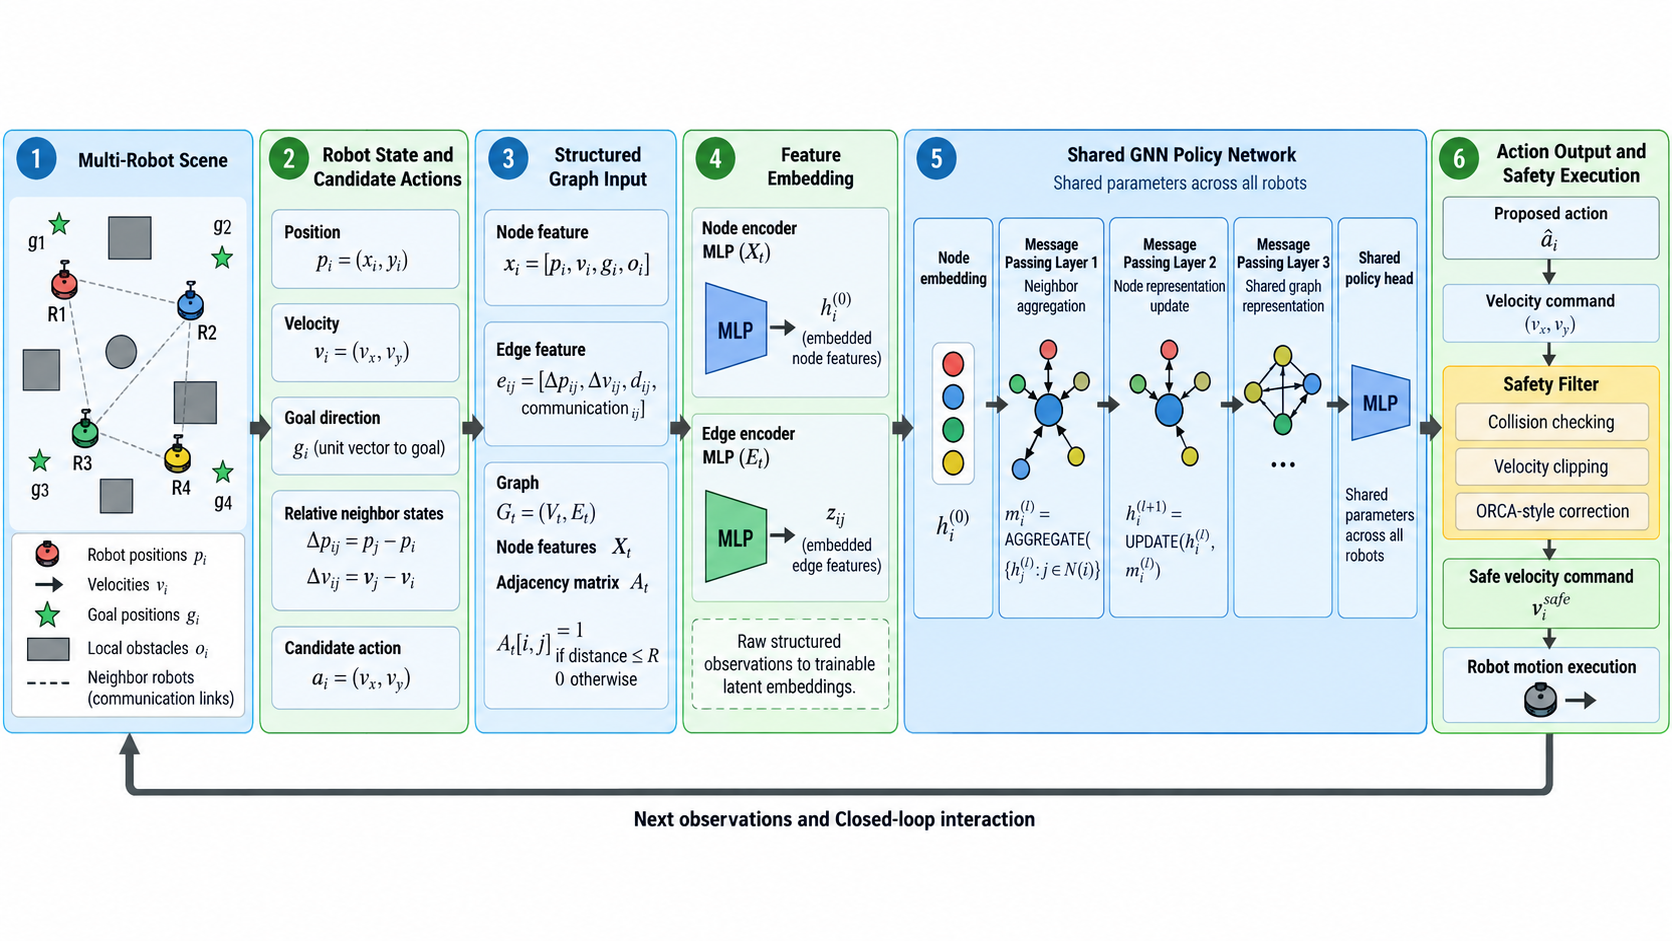
\includegraphics[width=\textwidth]{gnn_architecture_ai_fig1_draft_v2.png}
\caption{多机器人导航闭环：场景与状态观测、结构化图输入、特征嵌入、共享 GNN 推理以及动作输出与可选安全过滤。}
\label{fig:architecture}
\end{figure}

\subsection{基线方法}
本文实现 A* 网格路径跟踪、ORCA-style 局部排斥控制和一个无外部依赖的 RVO-style 候选速度控制器。RVO-style 控制器在有限速度方向和速度等级上枚举候选动作，根据预测邻居间距、障碍物占用和目标进度进行评分。由于该实现用于统一实验，文中将其称为 RVO-style，而不声称其等价于形式验证的标准 RVO 参考实现。

\subsection{MLP 与消息传递 GNN}
MLP 对每个节点独立应用相同的多层感知器，不接收邻接矩阵，用于区分节点特征本身和显式交互建模的贡献。GNN 首先通过线性层将节点特征映射为隐藏表示，每层对邻居表示进行平均聚合，并将自身表示与经过变换的邻居消息拼接后更新：
\begin{equation}
m_i^{(l)}=\frac{1}{\max(1,d_i)}\sum_j A_{ij}h_j^{(l)},\qquad
h_i^{(l+1)}=\sigma\left(W_l[h_i^{(l)}\Vert\phi_l(m_i^{(l)})]\right).
\end{equation}
加入边特征后，消息更新写为
\begin{equation}
 m_i^{(l)}=\frac{1}{\max(1,d_i)}\sum_j A_{ij}\left(\phi_l(h_j^{(l)})+\psi_l(e_{ij})\right),
 \quad h_i^{(l+1)}=\operatorname{ReLU}\left(W_l[h_i^{(l)}\Vert m_i^{(l)}]\right).
\end{equation}
本文使用 3 层消息传递、128 个隐藏单元和共享动作头。训练采用 ORCA-style 专家动作的模仿学习，动作通过 $\hat u_i=v_{max}\tanh(f_\theta(h_i))$ 约束在可执行范围内。

\subsection{联合训练目标}
仅用动作模仿损失会使策略复制专家的局部行为，却不一定保证闭环轨迹安全。本文使用四项损失的加权和：
\begin{equation}
 \mathcal{L}=\lambda_a\mathcal{L}_{act}+\lambda_c\mathcal{L}_{col}+\lambda_p\mathcal{L}_{prog}+\lambda_s\mathcal{L}_{smooth}.
\end{equation}
其中 $\mathcal{L}_{act}=\frac{1}{|\mathcal V|}\sum_i\operatorname{Huber}(u_i,u_i^*)$；令预测一步后距离为 $d_{ij}'=\|p_i+\Delta t u_i-p_j-\Delta t u_j\|$，碰撞惩罚为
\begin{equation}
 \mathcal{L}_{col}=\frac{1}{N(N-1)}\sum_{i\ne j}[d_{safe}-d_{ij}']_+^2.
\end{equation}
目标进度项和速度平滑项分别定义为
\begin{equation}
 \mathcal{L}_{prog}=\frac{1}{N}\sum_i[\|g_i-p_i'\|-\|g_i-p_i\|]_+,\qquad
 \mathcal{L}_{smooth}=\frac{1}{N}\sum_i\|u_i^t-u_i^{t-1}\|_2^2,
\end{equation}
其中 $[x]_+=\max(x,0)$。训练阶段对填充节点使用 mask $q_i\in\{0,1\}$，所有节点损失均替换为 $\sum_iq_i\ell_i/\max(1,\sum_iq_i)$。

\subsection{注意力模型与 Graph Transformer 对比}
为研究邻居加权机制和全局自注意力的影响，本文增加两个横向模型。Attention-GNN 使用与 GNN 相同的动态图和三层结构，但将均值聚合替换为基于查询、键和值的多头邻居注意力；注意力范围仍由局部邻接矩阵限制。Graph Transformer 使用多头自注意力、残差连接和前馈网络，并使用动态图邻接矩阵作为注意力掩码。两个模型均采用 128 个隐藏单元、4 个注意力头和共享策略头，输入、输出、训练数据及测试场景与 GNN 完全一致。

\subsection{边特征与多规模训练}
为增强动态图对避碰关系的表达能力，扩展模型为每条有向边加入五维特征，包括归一化相对位置、归一化相对速度和归一化接近速度。训练样本覆盖 5、10、20、30 和 40 个机器人以及四类地图，并将不同规模的图补齐到 40 个节点，通过节点掩码保证填充节点不参与损失计算。训练目标由动作模仿损失、一步碰撞惩罚、目标进度惩罚和速度平滑惩罚组成，使同一组共享参数能够处理可变规模机器人群体。

\subsection{安全过滤层}
在策略输出后，安全过滤器检查近距离机器人对的相对闭合速度，对存在风险的动作进行对称修正，再执行速度裁剪。该层作为策略外部约束进行单独消融，不将其效果混同为 GNN 本身的效果。
具体地，令 $\delta_{ij}=p_i-p_j$、$n_{ij}=\delta_{ij}/(\|\delta_{ij}\|+\epsilon)$。若 $\|\delta_{ij}\|<d_s+\tau$ 且 $(u_i-u_j)\cdot n_{ij}<0$，则施加对称修正
\begin{equation}
 \tilde u_i=u_i+\frac{\kappa_{ij}}{2}n_{ij},\quad
 \tilde u_j=u_j-\frac{\kappa_{ij}}{2}n_{ij},\quad
 \kappa_{ij}=-(u_i-u_j)\cdot n_{ij}+[d_s+\tau-\|\delta_{ij}\|]_+,
\end{equation}
随后执行 $\tilde u_i\leftarrow\operatorname{clip}(\tilde u_i,v_{max})$。该模块只在推理和 ROS 控制阶段启用。

\section{实验设计}
实验包含 crossing、open、random 和 narrow 四类地图，机器人数量为 5、10、20、30 和 40。开发数据集使用固定种子生成 20 个 episode，每个 episode 最多 160 个时间步；扩展测试使用种子 100--129，每种地图、模型和规模各 30 个 episode。数据以压缩 NPZ 保存，包含 features、adjacency、actions、positions、rewards、obstacles、layout、expert 和 episode\_step 字段。

扩展测试包含 $4\times5\times3\times30=1800$ 个安全过滤回合，分别覆盖三种学习模型、五种规模和四类地图。所有方法使用相同初始状态、目标、障碍物、动作限制和终止规则。评价指标包括目标到达率、严格无物理碰撞到达率、安全距离违规事件、物理碰撞事件、发生碰撞的 episode 比例、最小机器人间距、累计路径长度、最终目标误差和每个控制步的平均计算时间。安全距离违规阈值为 0.72 m，物理碰撞阈值为两个机器人半径之和，即 0.56 m；二者不混为同一指标。对每个比例指标报告跨 episode 的均值和标准差。

\section{实验结果}
\subsection{主实验比较}
表~\ref{tab:main} 汇总了四类地图上的聚合结果。RVO-style 的成功率较高且路径较短，但控制时间随机器人数量增长明显；ORCA-style 的碰撞事件平均值较低，但部分狭窄场景存在任务停滞；MLP 的成功率较高但碰撞风险明显；GNN 在部分 crossing 和 random 场景具有较好的协同行为，但跨地图稳定性仍不足。因此，不能仅依据成功率或路径长度宣称 GNN 全面优于传统基线。

\subsection{注意力与 Transformer 横向比较}
新增模型在 480 个学习策略回合上进行评估。GNN、Attention-GNN、Graph Transformer 和 MLP 的总体目标到达率分别为 0.683、0.342、0.558 和 0.817。Graph Transformer 的总体严格无物理碰撞到达率为 0.058，高于 GNN 的 0.008，但其控制时间约为 GNN 的 1.6 倍；Attention-GNN 的到达率明显下降，说明简单地引入注意力并不能保证性能提升。该结果表明，注意力机制的表达能力、训练分布和安全目标之间仍需要联合设计。

\begin{figure}[H]
\centering
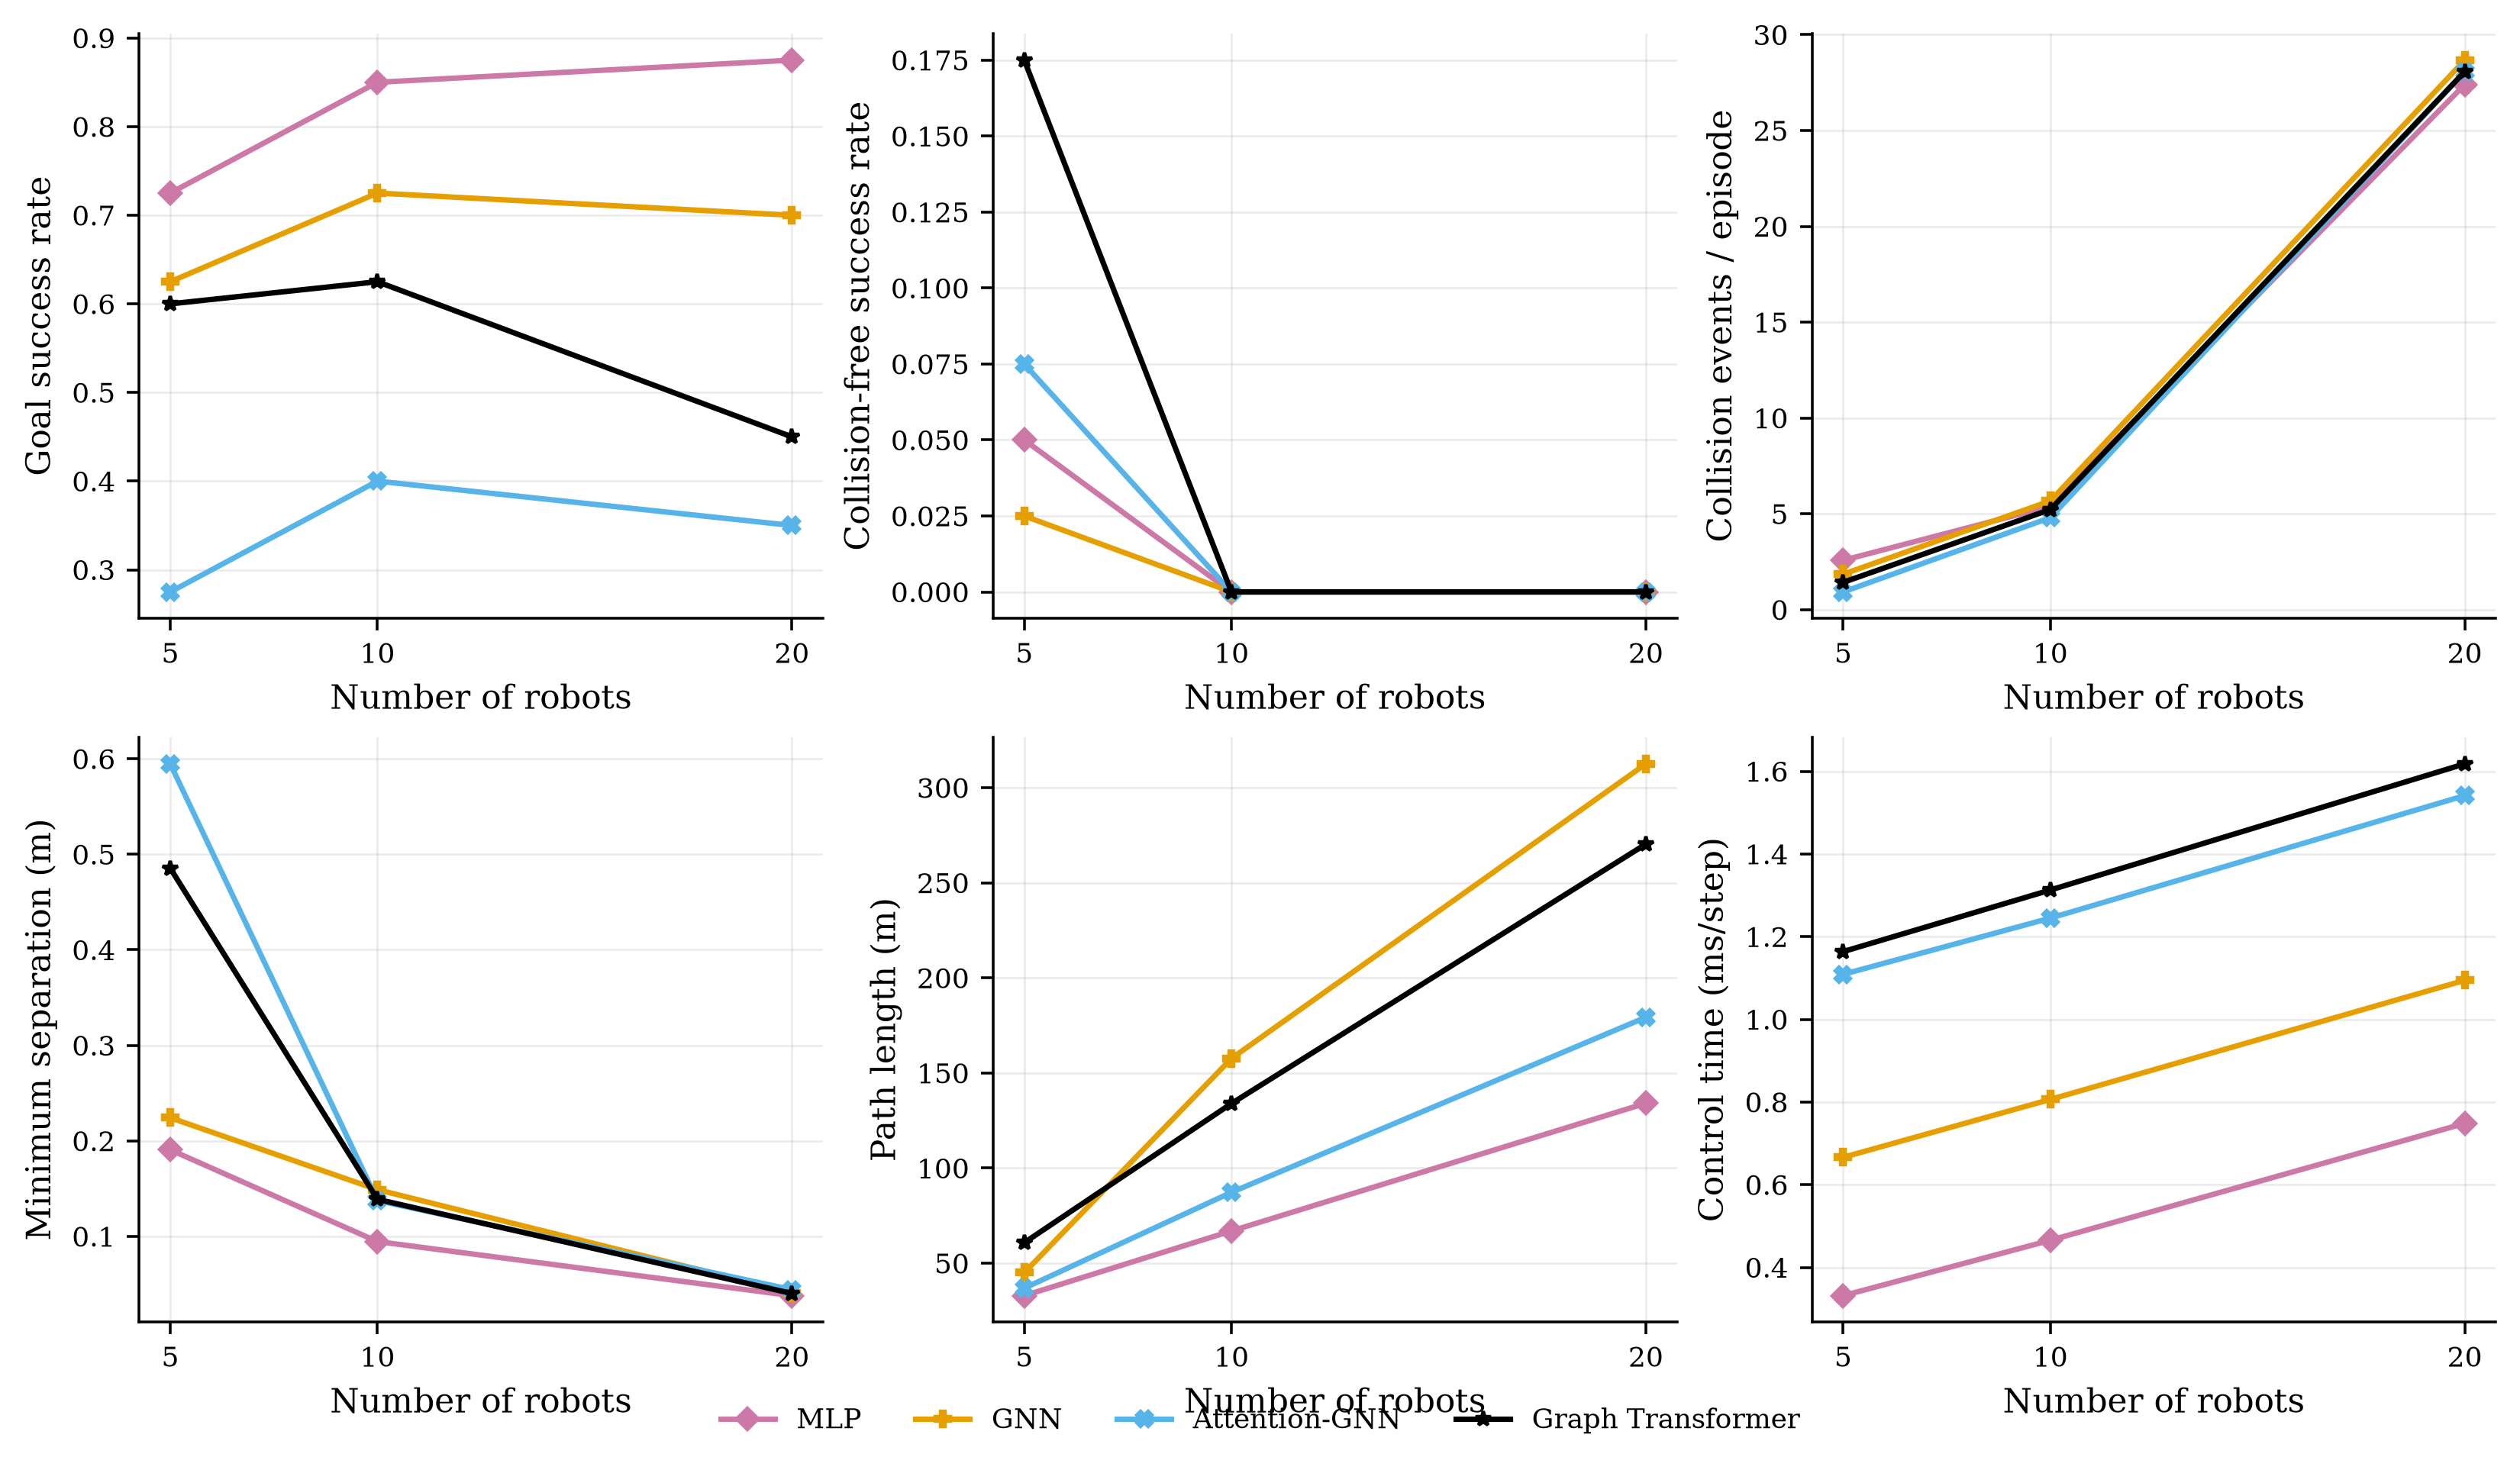
\includegraphics[width=0.98\textwidth]{extended_learned_models.png}
\caption{MLP、GNN、Attention-GNN 和 Graph Transformer 的横向比较。严格无碰撞成功率采用机器人物理直径阈值计算，安全距离违规单独报告。}
\label{fig:extended_models}
\end{figure}

\begin{table}[H]
\centering\small
\caption{学习模型横向比较的总体均值。}
\label{tab:learned_models}
\resizebox{\textwidth}{!}{\begin{tabular}{lrrrrrr}
\toprule
模型 & 成功率 & 无物理碰撞成功率 & 物理碰撞事件 & 安全违规事件 & 最小间距/m & 控制时间/ms\\
\midrule
MLP & 0.817 & 0.017 & 9.250 & 11.792 & 0.108 & 0.515\\
GNN & 0.683 & 0.008 & 8.825 & 12.067 & 0.138 & 0.856\\
Attention-GNN & 0.342 & 0.025 & 8.167 & 11.267 & 0.259 & 1.298\\
Graph Transformer & 0.558 & 0.058 & 8.833 & 11.575 & 0.221 & 1.365\\
\bottomrule
\end{tabular}}
\end{table}

\begin{table}[H]
\centering\small
\caption{主实验聚合结果。}
\label{tab:main}
\begin{tabular}{llrrrrr}
\toprule
方法 & 机器人 & 成功率 & 碰撞事件 & 最小间距/m & 路径长度/m & 控制时间/ms\\
\midrule
A* & 5 & 1.000 & 1.925 & 0.280 & 37.666 & 0.512\\
A* & 10 & 1.000 & 6.075 & 0.098 & 106.764 & 1.205\\
A* & 20 & 1.000 & 30.700 & 0.035 & 216.192 & 2.493\\
MLP & 5 & 0.725 & 2.575 & 0.191 & 32.927 & 0.342\\
MLP & 10 & 0.850 & 5.400 & 0.095 & 66.957 & 0.483\\
MLP & 20 & 0.875 & 27.400 & 0.038 & 134.094 & 0.775\\
GNN & 5 & 0.625 & 1.850 & 0.224 & 45.026 & 0.683\\
GNN & 10 & 0.725 & 5.675 & 0.149 & 157.656 & 0.828\\
GNN & 20 & 0.700 & 28.675 & 0.041 & 312.528 & 1.129\\
ORCA-style & 5 & 0.775 & 1.425 & 0.396 & 43.519 & 0.213\\
ORCA-style & 10 & 0.825 & 3.825 & 0.296 & 123.110 & 0.486\\
ORCA-style & 20 & 0.825 & 13.500 & 0.230 & 274.271 & 1.303\\
RVO-style & 5 & 0.975 & 1.825 & 0.294 & 29.003 & 7.779\\
RVO-style & 10 & 1.000 & 5.575 & 0.131 & 63.525 & 24.941\\
RVO-style & 20 & 1.000 & 23.325 & 0.062 & 127.577 & 87.373\\
\bottomrule
\end{tabular}
\end{table}

\begin{figure}[H]
\centering
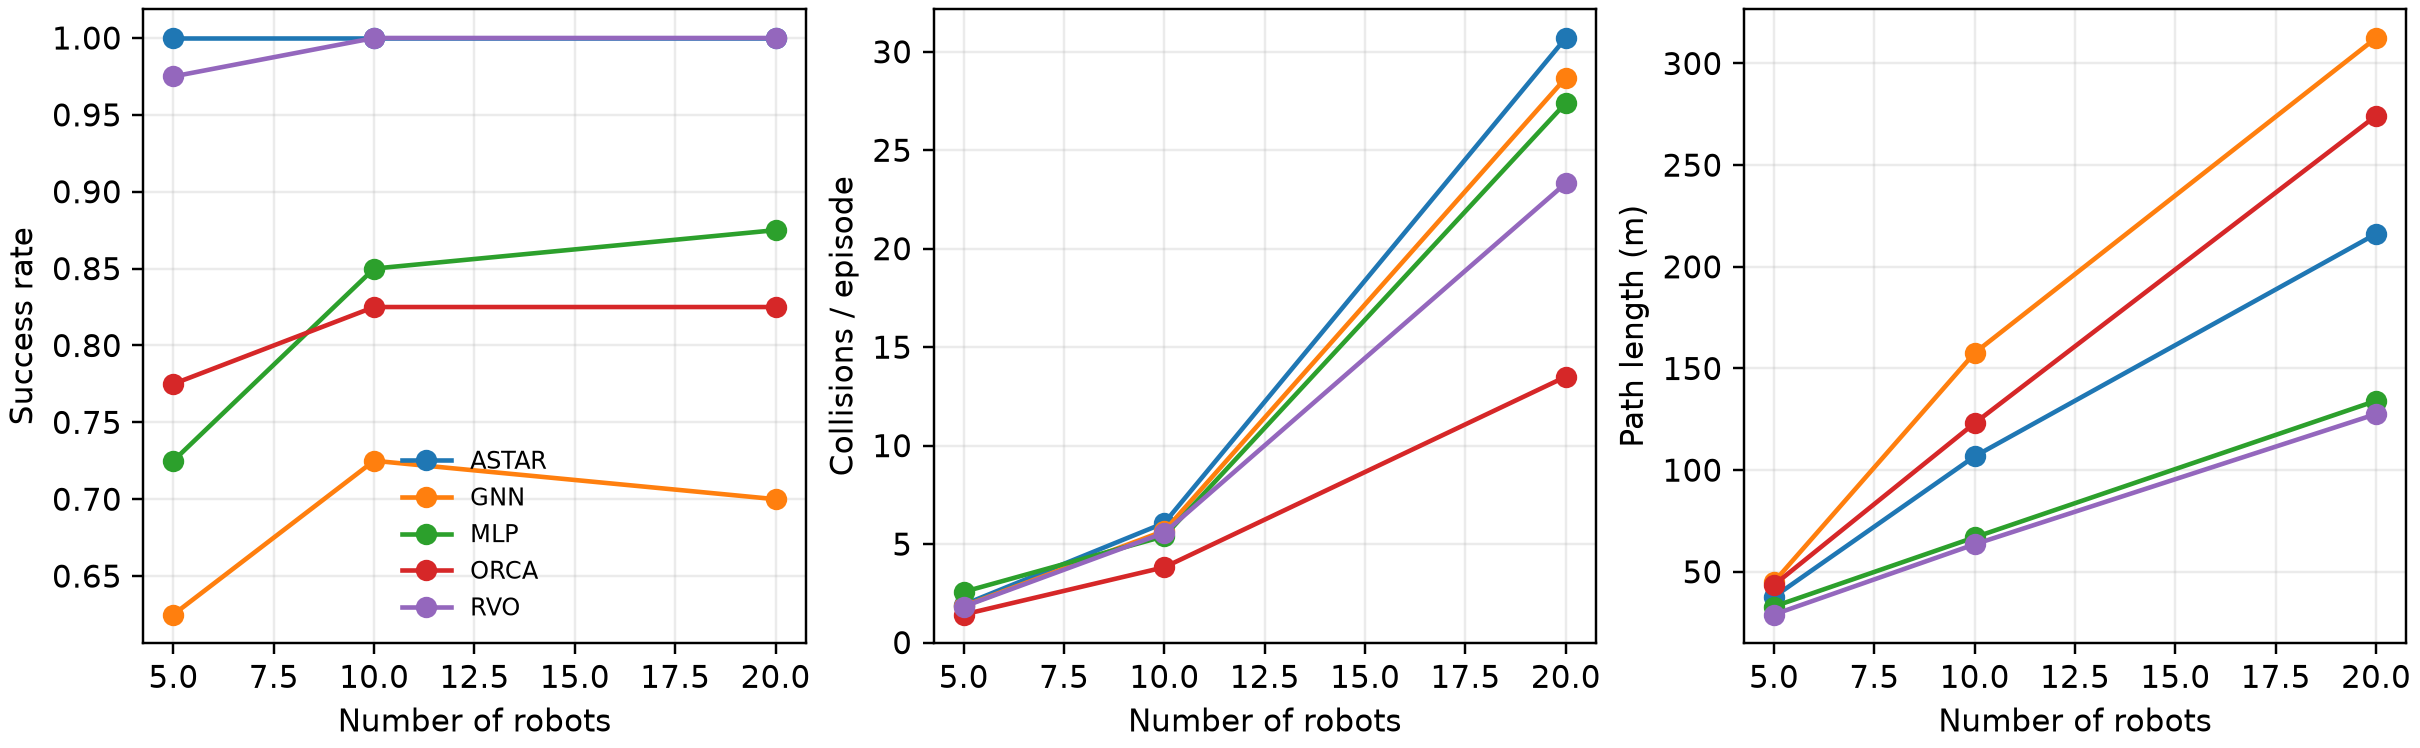
\includegraphics[width=0.98\textwidth]{baselines_final.png}
\caption{不同方法在不同机器人规模下的综合比较。}
\label{fig:baselines}
\end{figure}

\subsection{图结构消融}
在 10 个机器人时，局部图的平均成功率为 0.725，无边模型为 0.425；在 20 个机器人时，局部图为 0.700，无边模型为 0.425。该结果支持消息传递对协同决策有实际贡献，但局部图和全局图仍存在碰撞事件，说明图表示本身不能替代安全约束。

\begin{figure}[H]
\centering
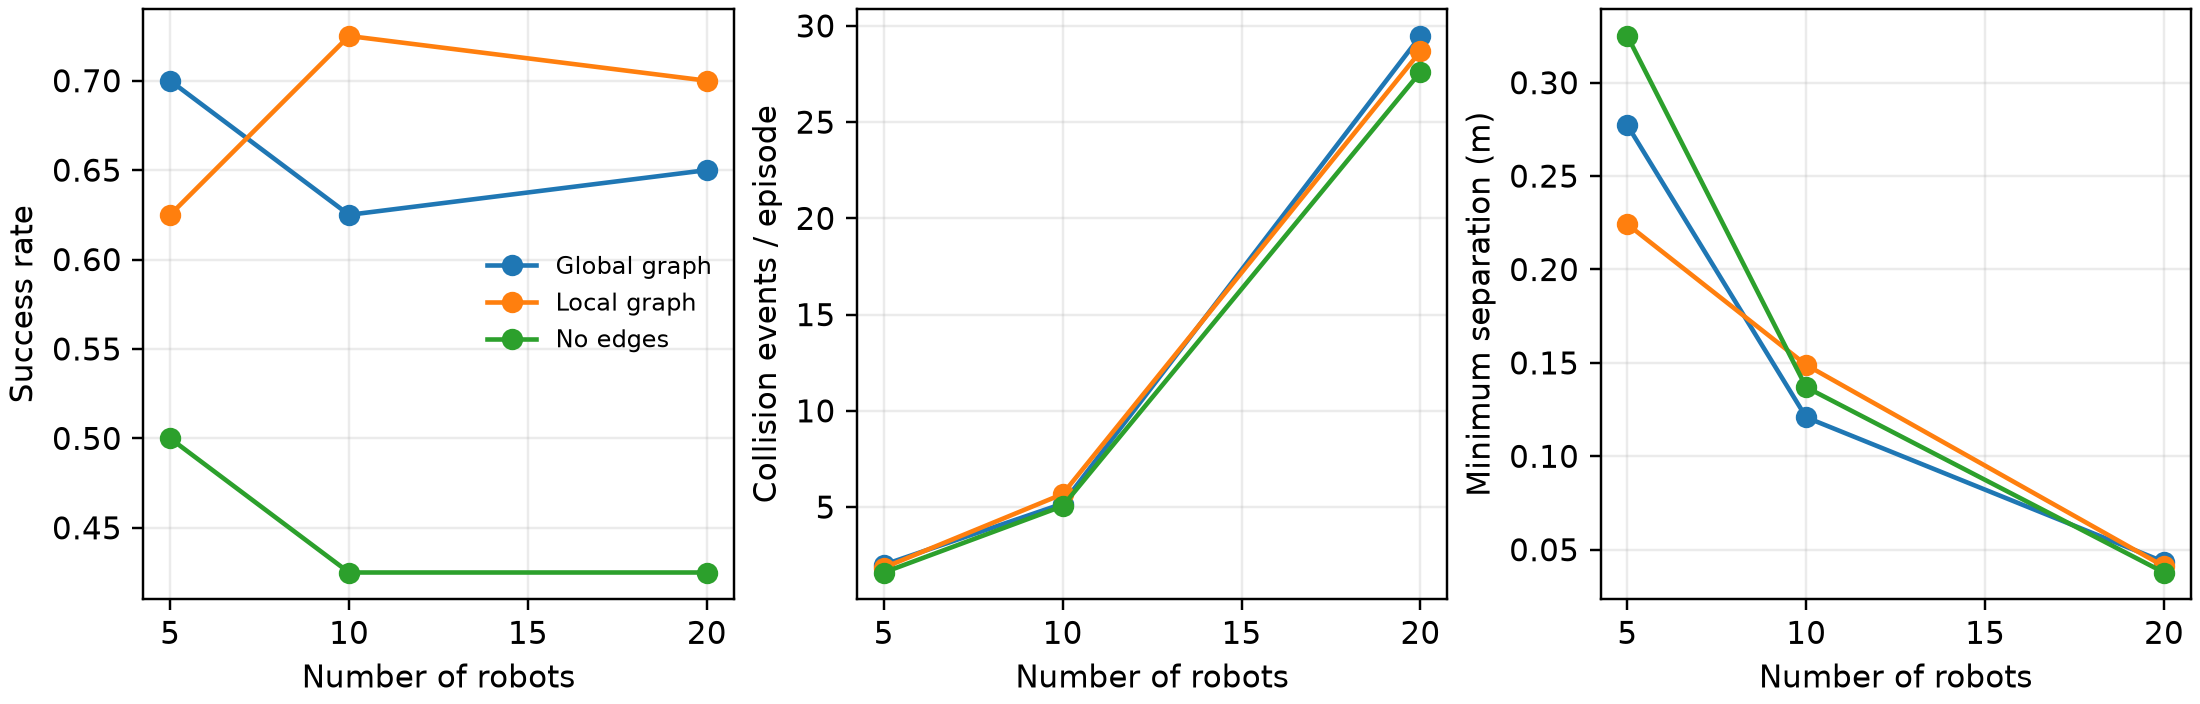
\includegraphics[width=0.92\textwidth]{ablation_graph_final.png}
\caption{无边、局部图和全局图的结构消融结果。}
\label{fig:graph_ablation}
\end{figure}

\subsection{安全层消融}
物理碰撞重算显示，安全层在 10 个机器人时将平均物理碰撞事件从 4.3 降至 0.1，并将严格无物理碰撞成功率提高到 0.8；在 20 个机器人时，物理碰撞事件从 18.0 降至 3.8，但仍未实现稳定的无碰撞到达。安全层可能造成部分机器人停滞，体现出安全性和任务完成率之间的直接权衡；更理想的方案是将安全约束纳入训练目标。

\begin{figure}[H]
\centering
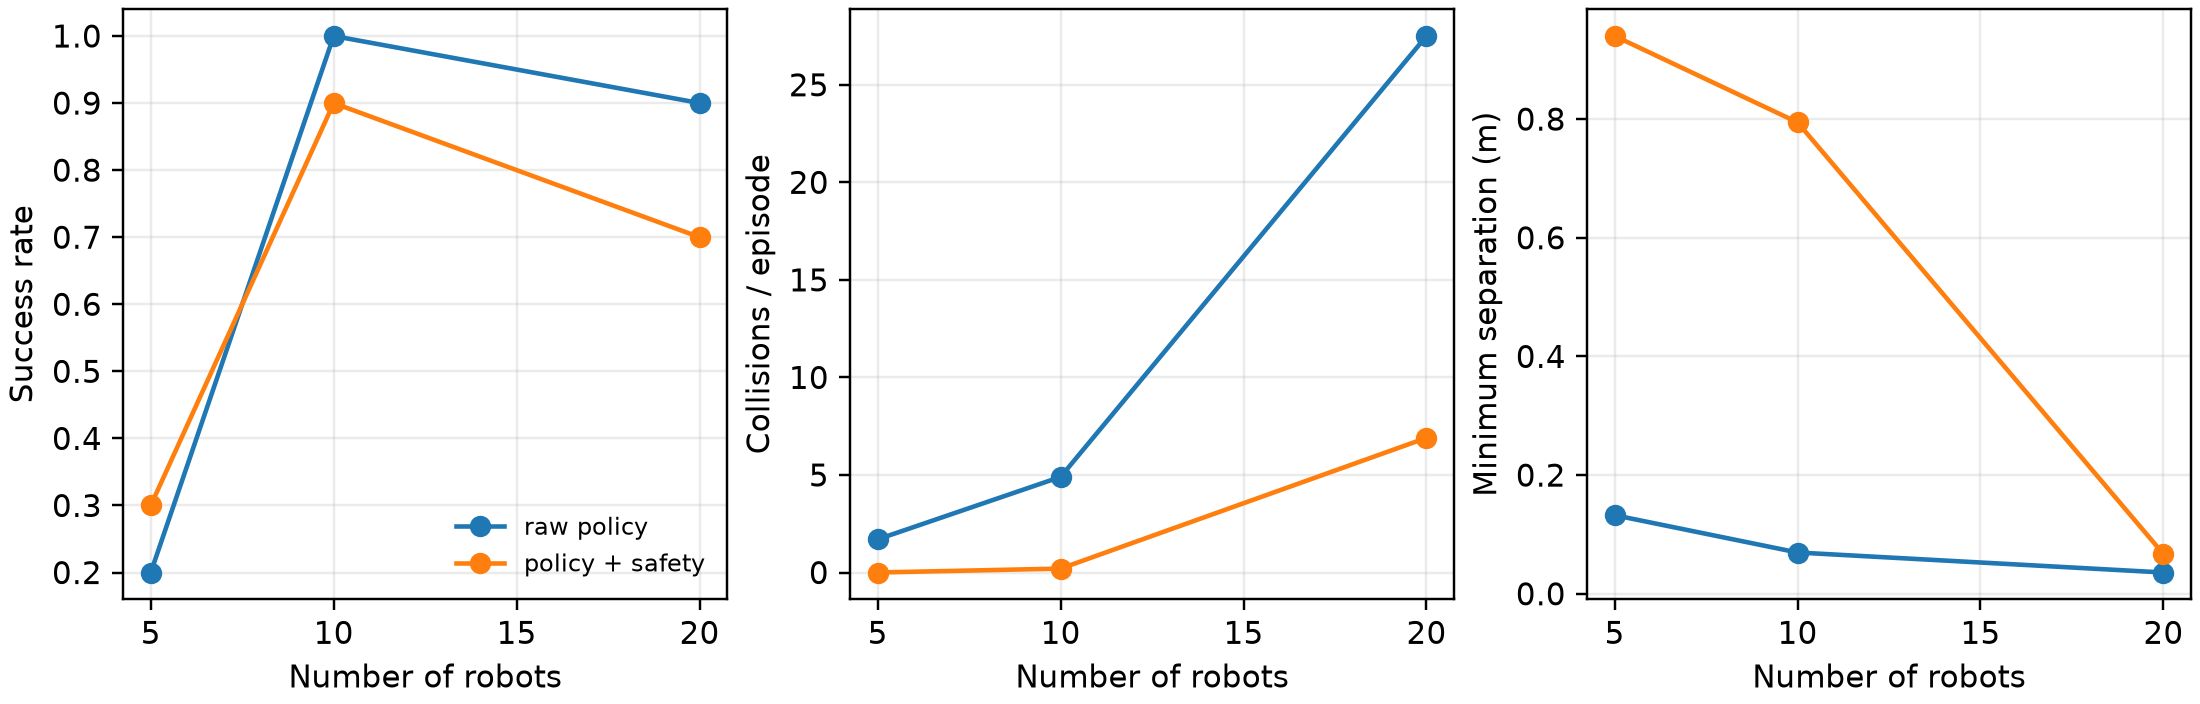
\includegraphics[width=0.92\textwidth]{ablation_safety_final.png}
\caption{安全过滤层消融结果。}
\label{fig:safety_ablation}
\end{figure}

\subsection{通信半径、泛化与轨迹}
通信半径增大后平均图度增加，能够提供更多邻居信息，但也会增加消息聚合开销。在物理碰撞消融中，半径 2.0 m 在 10 个机器人时成功率仅为 0.2，而半径 3.4 m 和 5.5 m 分别达到 1.0；全局图达到 0.9，但并未消除物理碰撞。三个独立 GNN checkpoint 的 5、10、20 机器人平均成功率分别为 0.517、0.767 和 0.850，标准差分别为 0.388、0.161 和 0.115，5 机器人结果方差较大，说明当前训练配置仍需改进。

\begin{figure}[H]
\centering
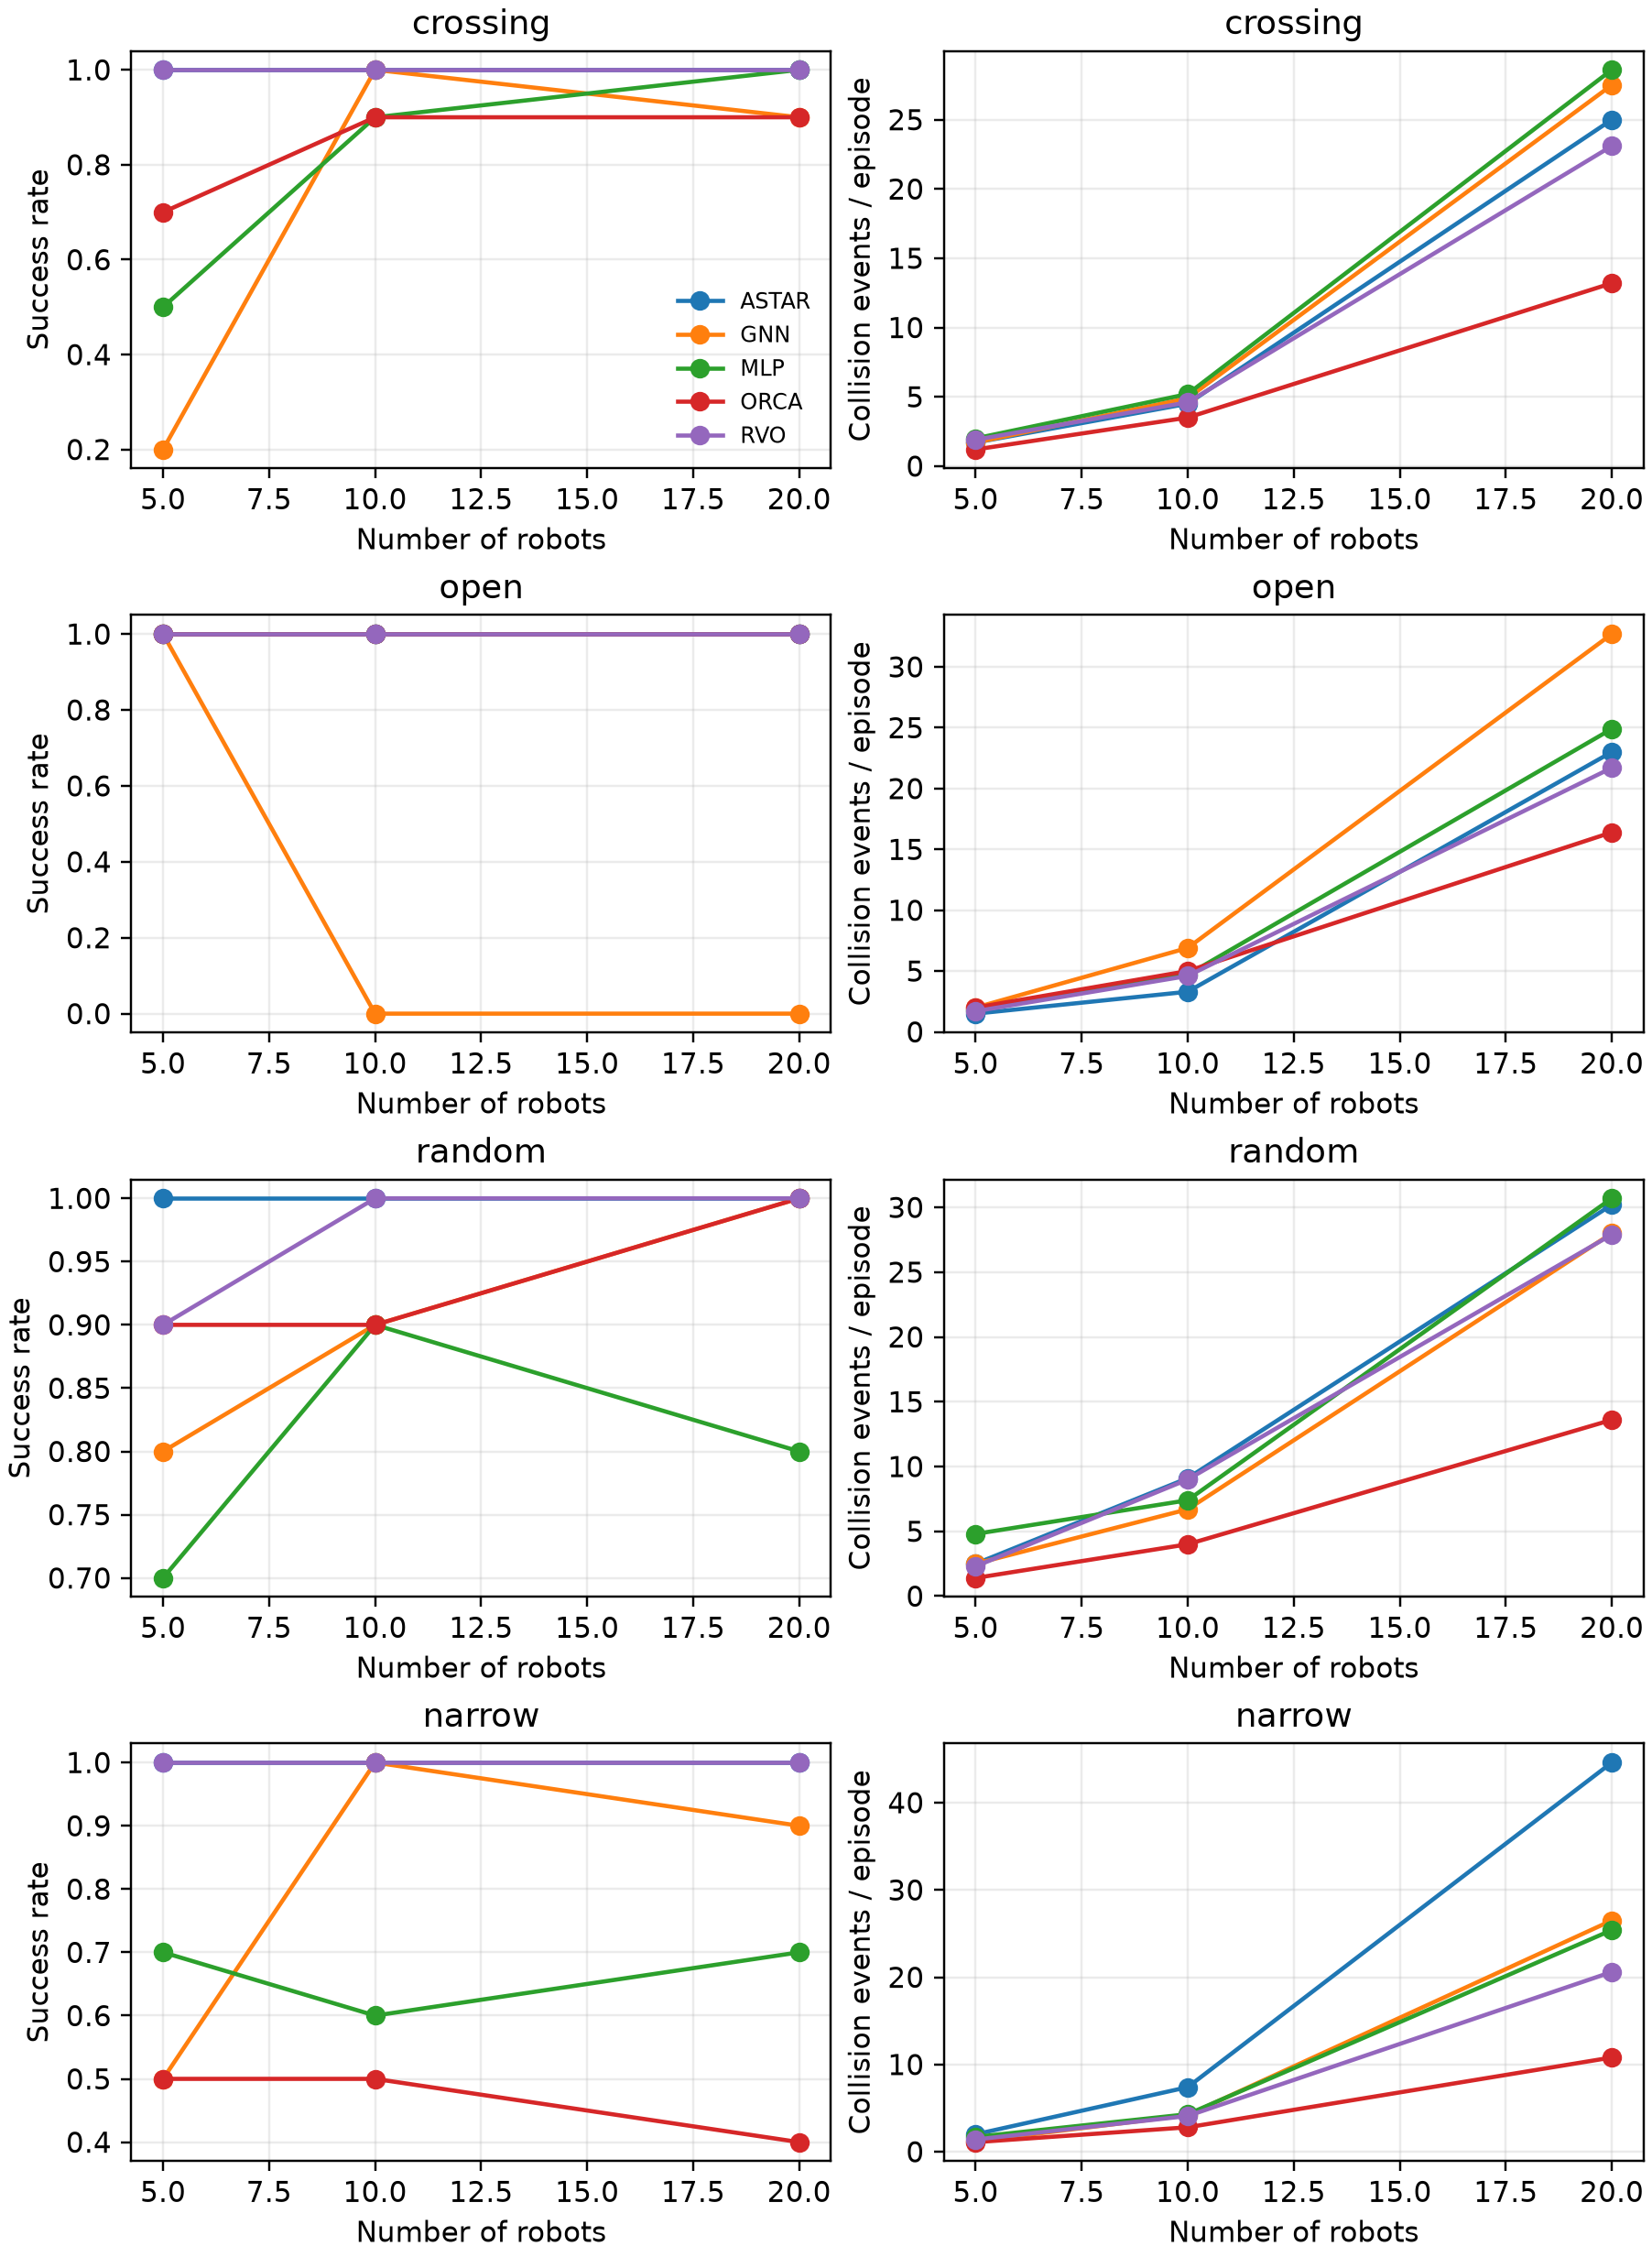
\includegraphics[width=0.49\textwidth]{generalization_final.png}\hfill
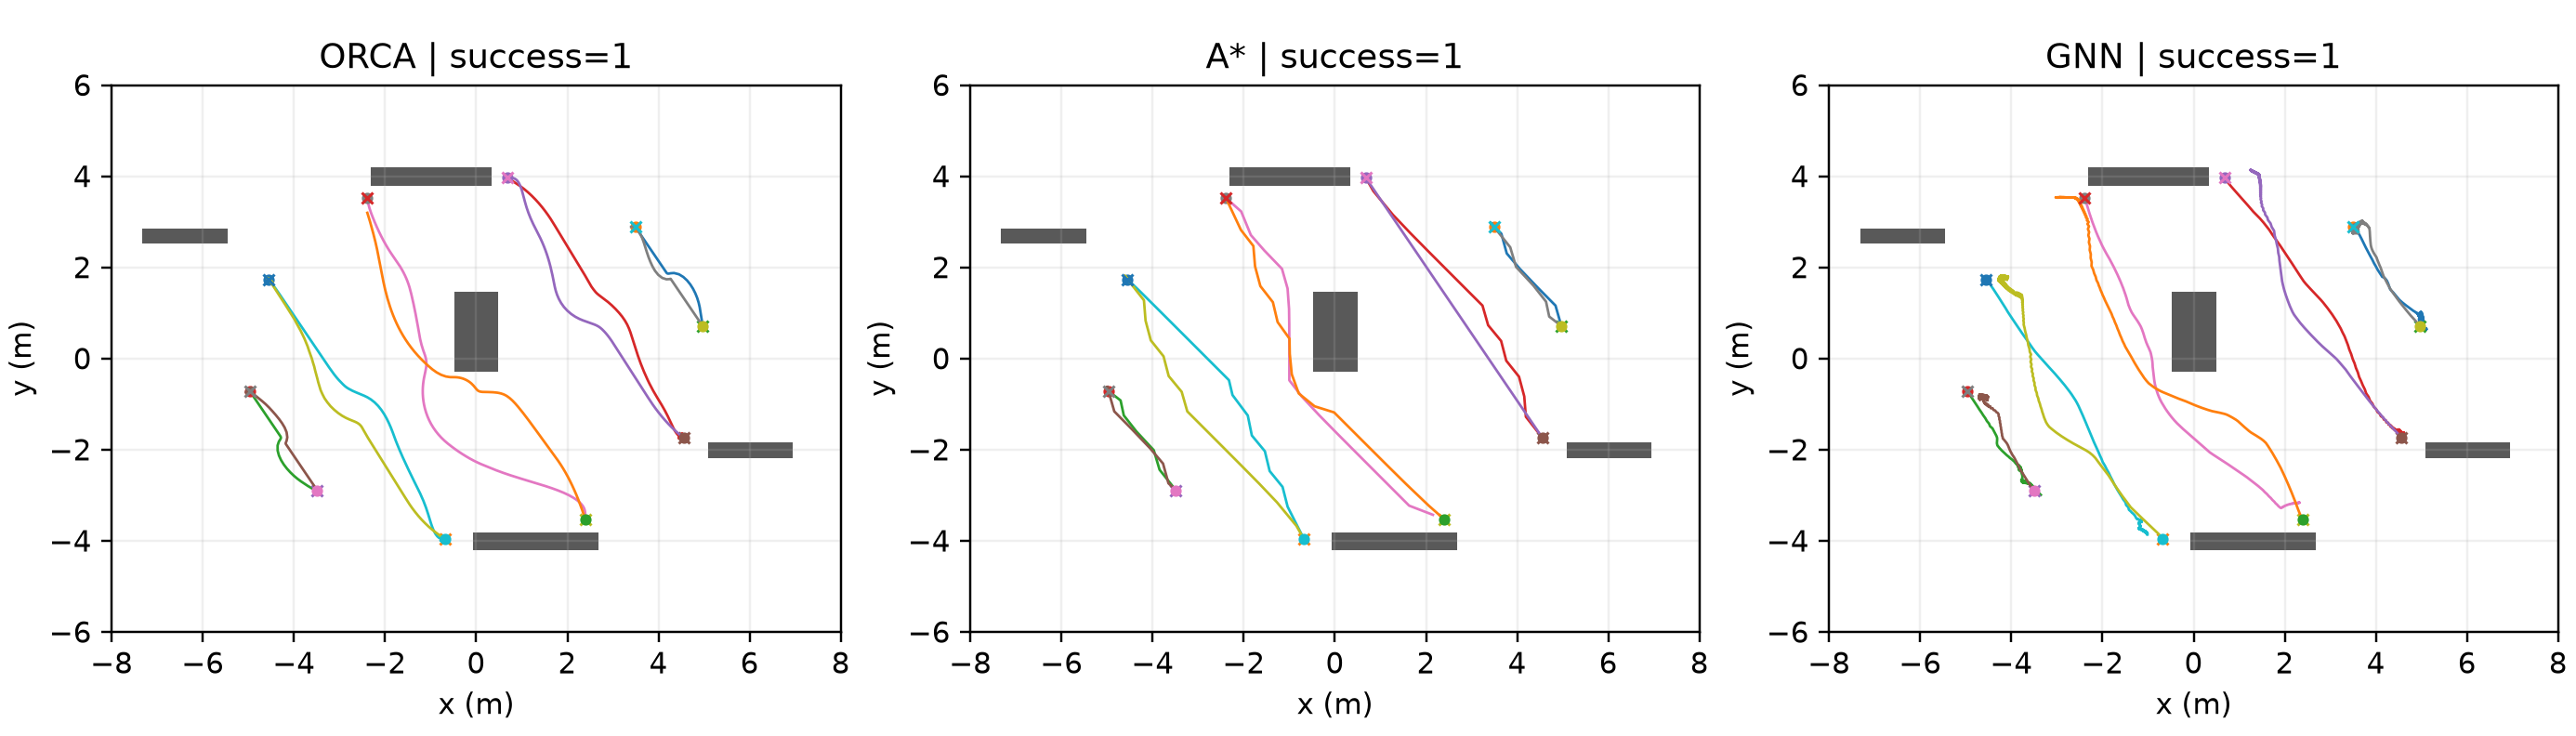
\includegraphics[width=0.49\textwidth]{trajectories_final.png}
\caption{跨规模泛化结果与典型轨迹。}
\label{fig:generalization}
\end{figure}

\begin{figure}[H]
\centering
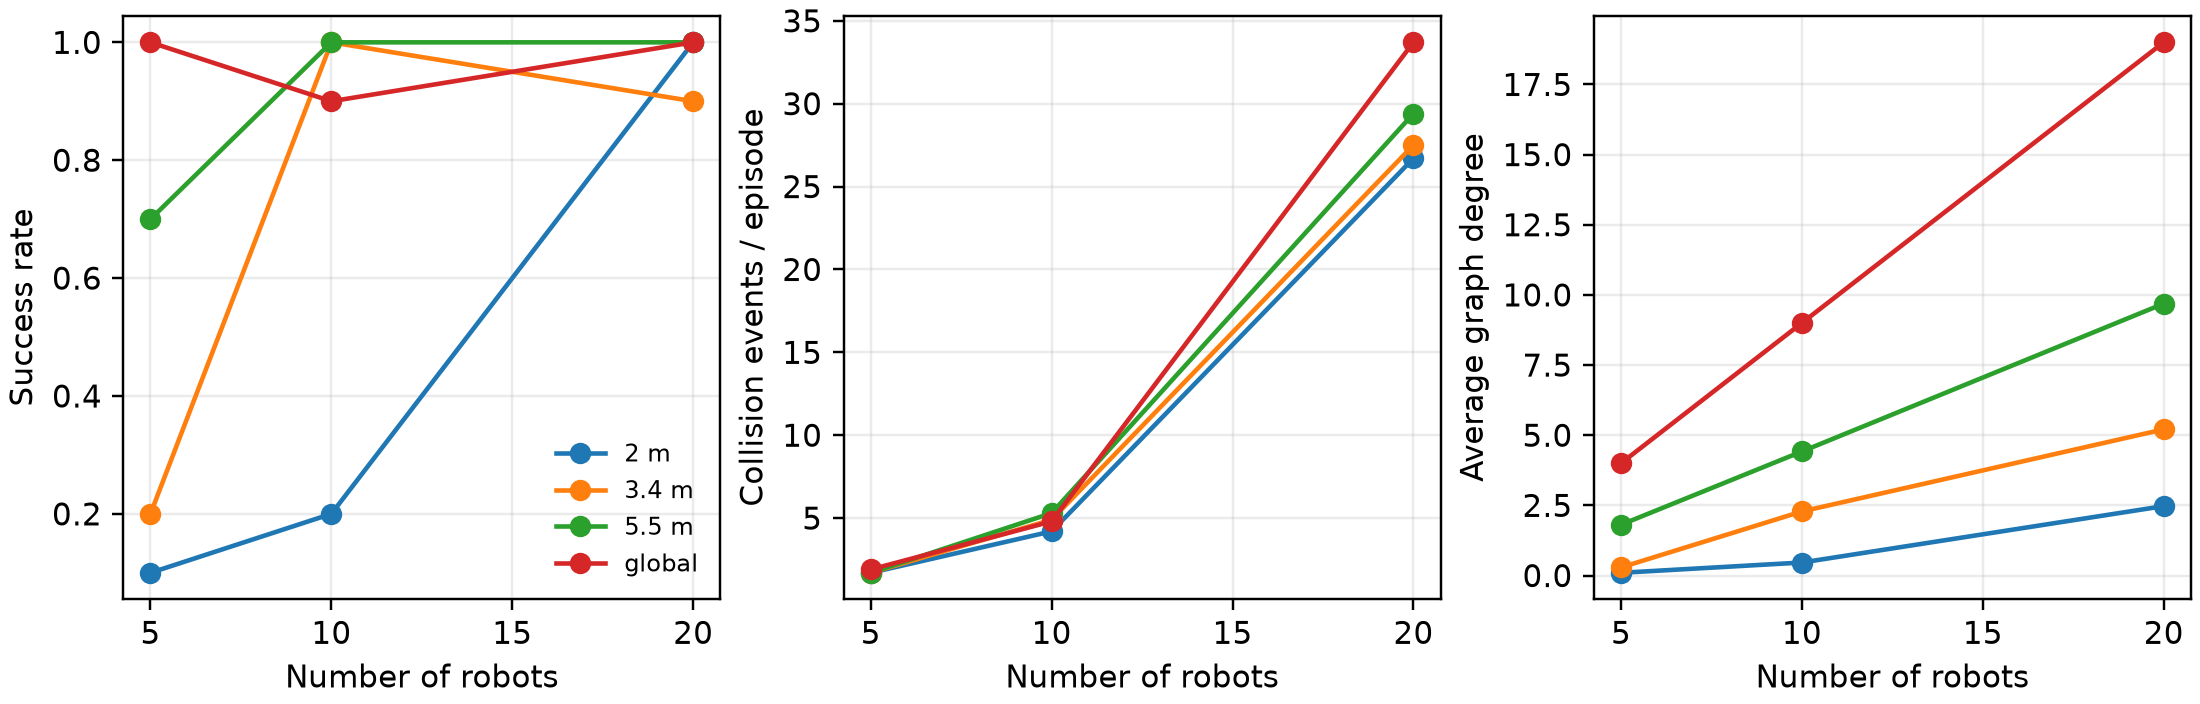
\includegraphics[width=0.92\textwidth]{ablation_radius_physical.png}
\caption{通信半径对成功率、碰撞事件和图度的影响。}
\label{fig:radius_ablation}
\end{figure}

\subsection{多规模压力测试}
在 30 个未见测试种子上，扩展数据集共评估 1,800 个回合。未加安全过滤时，GNN 在 5、10、20、30 和 40 个机器人上的目标到达率分别为 0.992、0.992、0.975、0.983 和 1.000；Graph Transformer 分别为 0.983、1.000、1.000、1.000 和 1.000。然而，30 和 40 个机器人时两类模型的无物理碰撞成功率均接近 0，说明高到达率不能替代安全性指标。加入安全过滤后，GNN 在 20、30 和 40 个机器人上的无物理碰撞成功率分别为 0.708、0.250 和 0.000，Graph Transformer 分别为 0.767、0.242 和 0.017。因此，当前系统的实用工作区间约为 10--20 个机器人，30--40 个机器人更适合作为高密度压力测试。

表~\ref{tab:multiscale} 给出四类地图聚合后的安全过滤结果。Graph Transformer 在 10 个机器人时严格成功率为 1.000，但控制时间高于 GNN；当规模增至 30 和 40 时，三种模型均出现明显退化。GNN 在 5--20 个机器人区间的控制时间最低，且 20 个机器人时严格成功率达到 0.708，体现出效率和安全性的折中。图~\ref{fig:scaling} 进一步显示，最小间距随密度增大而下降，而控制时间总体增加；图~\ref{fig:heatmap} 说明 random 和 narrow 地图对高密度策略更具挑战性。

\begin{table}[H]
\centering\small
\caption{安全过滤后的多规模测试结果（四类地图均值）。}
\label{tab:multiscale}
\resizebox{\textwidth}{!}{\begin{tabular}{llrrrrr}
\toprule
模型 & 机器人 & 到达率 & 严格成功率 & 物理碰撞事件 & 最小间距/m & 控制时间/ms\\
\midrule
GNN & 5 & 0.967 & 0.967 & 0.000 & 0.974 & 0.890\\
GNN & 10 & 0.958 & 0.958 & 0.000 & 0.953 & 1.035\\
GNN & 20 & 0.758 & 0.708 & 0.075 & 0.869 & 1.369\\
GNN & 30 & 0.400 & 0.250 & 1.158 & 0.608 & 1.704\\
GNN & 40 & 0.042 & 0.000 & 6.883 & 0.406 & 2.066\\
Attention-GNN & 5 & 0.925 & 0.925 & 0.000 & 1.000 & 1.273\\
Attention-GNN & 10 & 0.850 & 0.850 & 0.000 & 0.931 & 1.423\\
Attention-GNN & 20 & 0.358 & 0.283 & 0.425 & 0.746 & 1.759\\
Graph Transformer & 5 & 0.983 & 0.983 & 0.000 & 0.998 & 1.497\\
Graph Transformer & 10 & 1.000 & 1.000 & 0.000 & 0.938 & 1.646\\
Graph Transformer & 20 & 0.842 & 0.767 & 0.217 & 0.795 & 1.991\\
Graph Transformer & 30 & 0.467 & 0.242 & 2.267 & 0.560 & 2.329\\
Graph Transformer & 40 & 0.108 & 0.017 & 9.025 & 0.335 & 2.691\\
\bottomrule
\end{tabular}}
\end{table}

\begin{figure}[H]
\centering
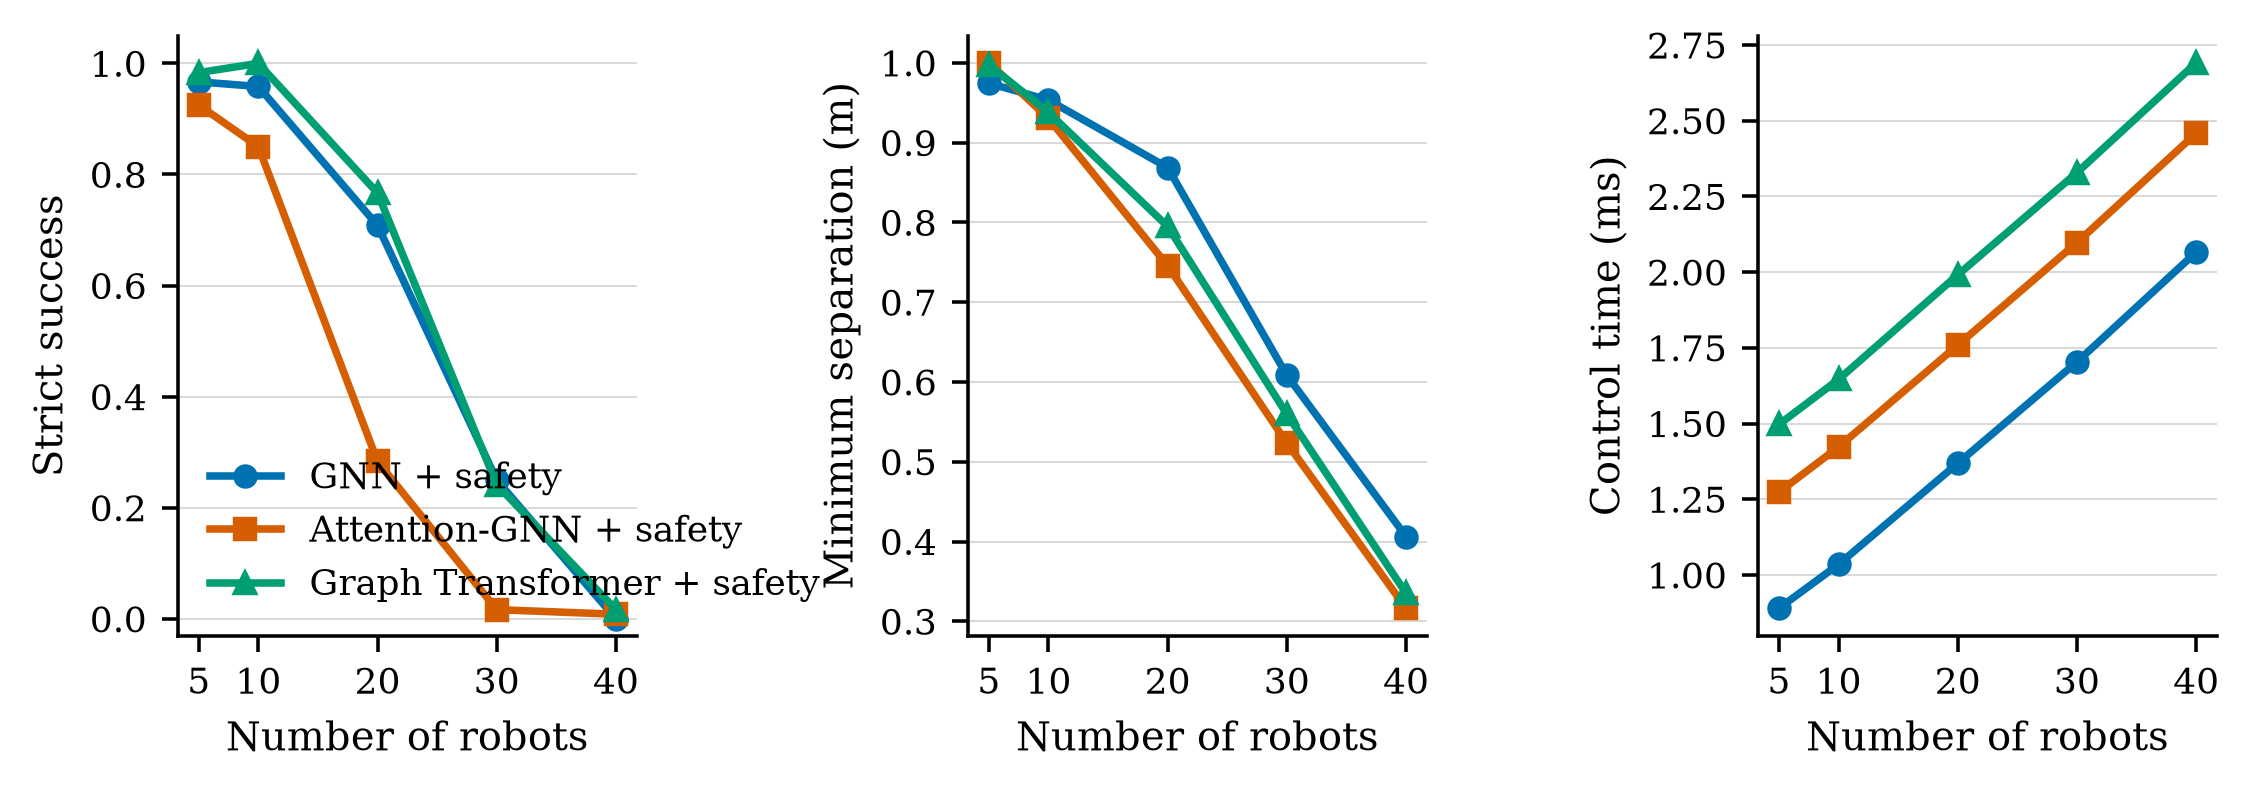
\includegraphics[width=\textwidth]{multiscale_safety_scaling.png}
\caption{不同机器人规模下的严格成功率、最小间距和控制时间。}
\label{fig:scaling}
\end{figure}

\begin{figure}[H]
\centering
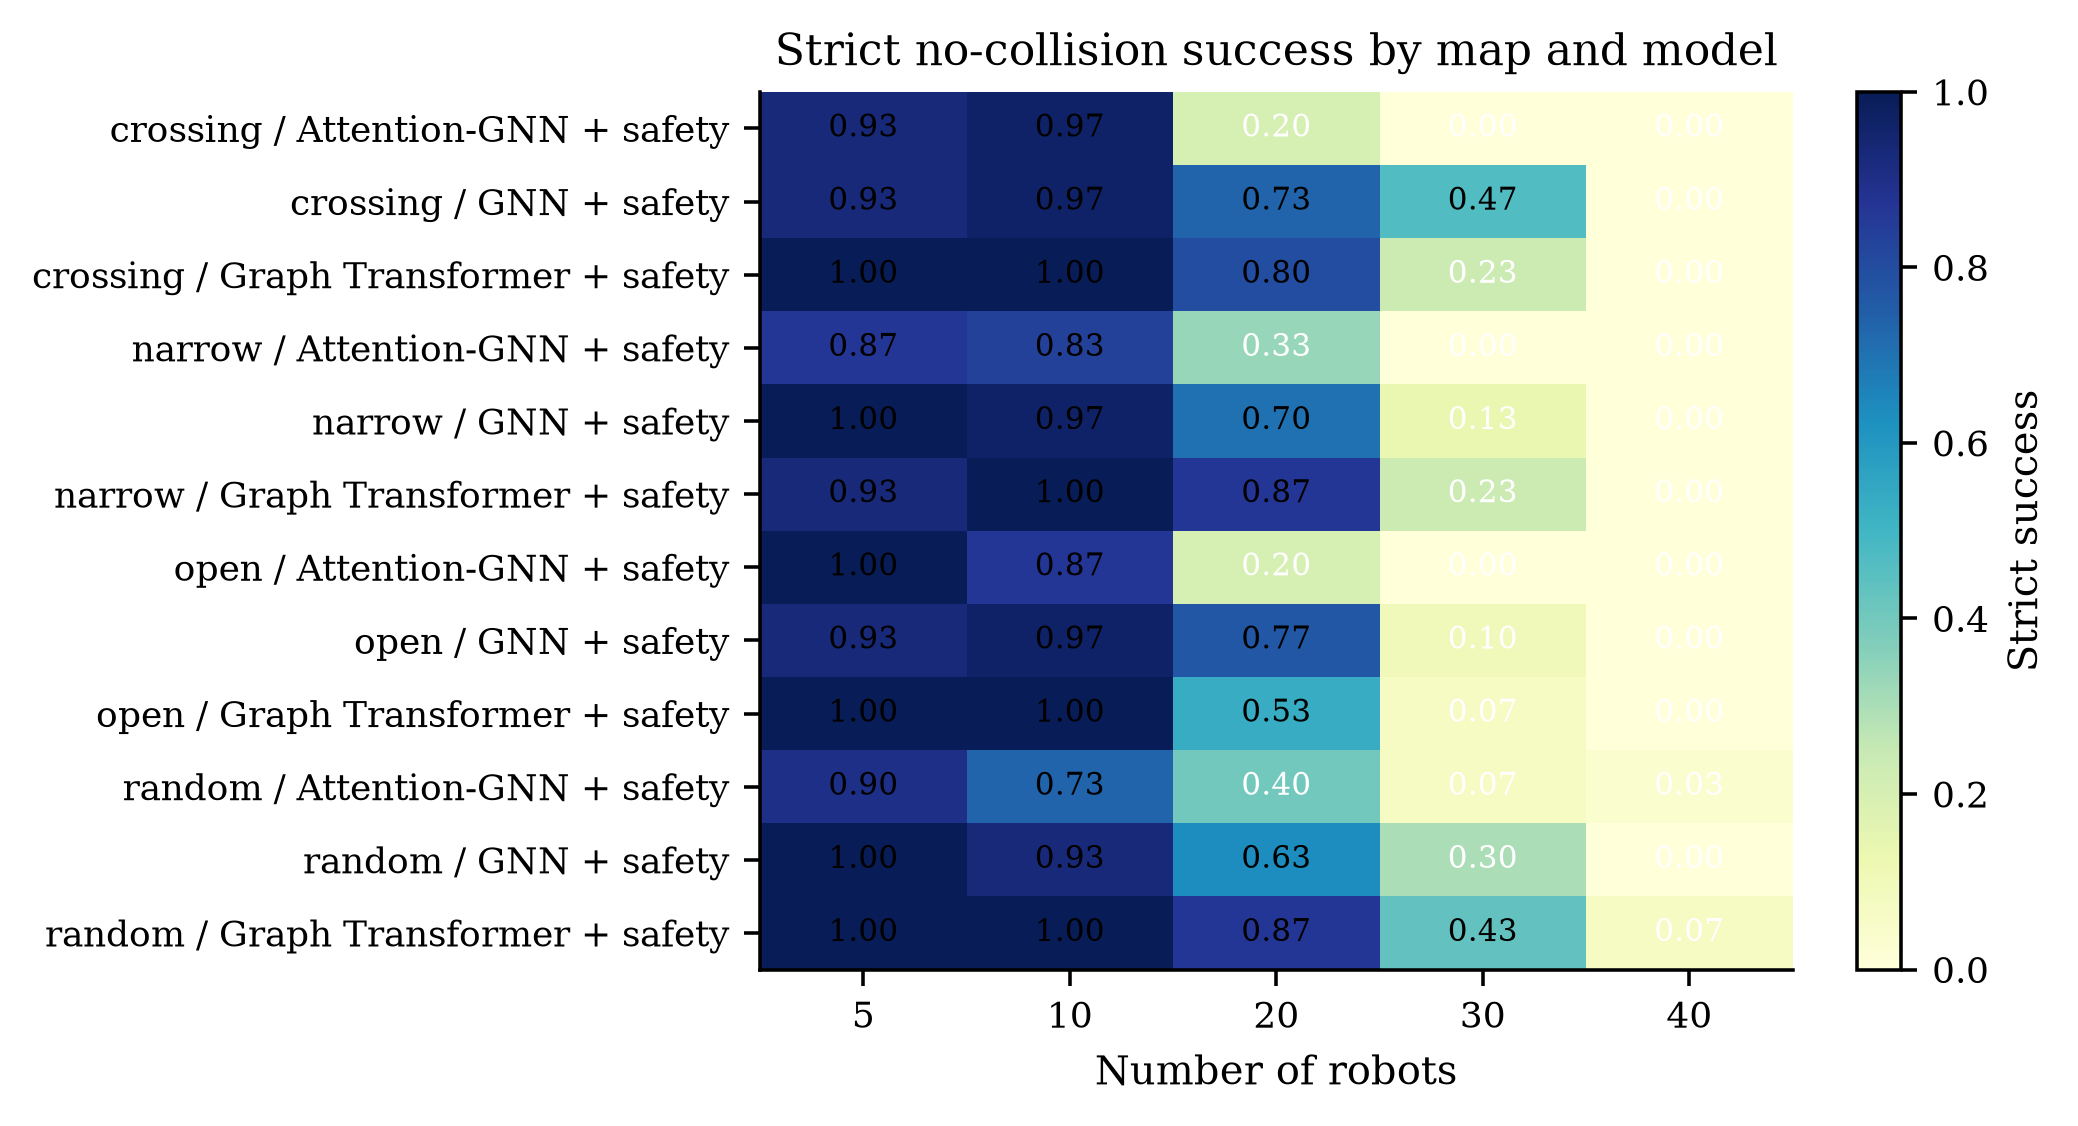
\includegraphics[width=0.94\textwidth]{multiscale_map_heatmap.png}
\caption{四类地图与不同机器人规模下的严格无碰撞成功率热力图。}
\label{fig:heatmap}
\end{figure}

\section{ROS 2 与可视化验证}
本文提供 Tkinter 二维界面，可切换 ORCA、RVO、A*、MLP 和 GNN，并实时显示机器人、目标、通信边、轨迹和指标。ROS 2 适配器接入 Wheeltec 模型，在 3 个命名空间下验证了 /robot\_i/odom、/robot\_i/scan 和 /robot\_i/cmd\_vel。Marker 可视化节点发布 /multi\_robot/markers，RViz2 可显示机器人、目标、轨迹和通信边。启动命令如下：
\begin{verbatim}
cd /ds1/workspace/paper/multi_robot_gnn
bash ros2/run_multi_robot_gnn.sh 5 results/checkpoints/gnn_n10.npz true
\end{verbatim}

\section{局限性与讨论}
第一，RVO-style 控制器是本文为统一实验编写的有限速度候选方法，不是经过形式验证的标准 RVO 库实现。第二，扩展 GNN 虽然在 5--40 个机器人上进行多规模训练，但 30--40 个机器人时无碰撞到达率仍明显下降。第三，高密度场景的碰撞事件仍然较多，安全过滤会造成部分机器人停滞。第四，Gazebo 验证证明了 ROS 接口和可视化链路，但不能替代真实机器人实验。第五，当前工作使用模仿学习，尚未完成带有长期目标进度和严格安全约束的强化学习微调。

\section{结论}
本文构建了一个面向多机器人协同路径规划的动态图 GNN 实验与部署框架。实验表明，局部消息传递能够改善独立节点策略的协同性，安全过滤能够显著改善间距指标，但成功率、碰撞风险和通信计算开销之间存在明显权衡。后续工作应围绕更可靠的 RVO 参考实现、安全约束训练、跨地图泛化和真实机器人验证展开。

\bibliographystyle{plain}
\bibliography{../references}

\end{document}
